%%% LaTeX Template: Article/Thesis/etc. with colored headings and special fonts
%%%
%%% Source: http://www.howtotex.com/
%%% Feel free to distribute this template, but please keep to referal to http://www.howtotex.com/ here.
%%% February 2011
%%%
%%% Modified January 2016 by CDM

%%%  Preamble
\documentclass[11pt,letterpaper]{article}
\usepackage[margin=1.0in]{geometry}
\usepackage[T1]{fontenc}
\usepackage[bitstream-charter]{mathdesign}
\usepackage[latin1]{inputenc}					
\usepackage{amsmath}						
\usepackage{xcolor}
\usepackage{cite}
\usepackage{hyphenat}
\usepackage{graphicx}
\usepackage{float}
\usepackage{subfigure}
\usepackage{sectsty}
\usepackage[compact]{titlesec} 
\usepackage[tablegrid]{vhistory}
\usepackage{pbox}
\allsectionsfont{\color{accentcolor}\scshape\selectfont}

%%% Definitions
\definecolor{accentcolor}{rgb}{0.0,0.0,0.5} 
\newcommand{\teamname}{Project Iris}
\newcommand{\productname}{Iris}
\newcommand{\coursename}{CSE 4316: Senior Design II}
\newcommand{\semester}{Fall 2016}
\newcommand{\docname}{Arcitectural Design Specification}
\newcommand{\department}{Department of Computer Science \& Engineering}
\newcommand{\university}{The University of Texas at Arlington}
\newcommand{\authors}{Neil Simmons \\ Tyler D'Spain \\ Matthew Zielke \\ Syed Uddin \\ Tony McDonald}

%%% Headers and footers
\usepackage{fancyhdr}
	\pagestyle{fancy}						% Enabling the custom headers/footers
\usepackage{lastpage}	
	% Header (empty)
	\lhead{}
	\chead{}
	\rhead{}
	% Footer
	\lfoot{\footnotesize \teamname \ - \semester}
	\cfoot{}
	\rfoot{\footnotesize page \thepage\ of \pageref{LastPage}}	% "Page 1 of 2"
	\renewcommand{\headrulewidth}{0.0pt}
	\renewcommand{\footrulewidth}{0.4pt}

%%% Change the abstract environment
\usepackage[runin]{abstract}			% runin option for a run-in title
%\setlength\absleftindent{30pt}			% left margin
%\setlength\absrightindent{30pt}		% right margin
\abslabeldelim{\quad}	
\setlength{\abstitleskip}{-10pt}
\renewcommand{\abstractname}{}
\renewcommand{\abstracttextfont}{\color{accentcolor} \small \slshape}	% slanted text

%%% Start of the document
\begin{document}

%%% Cover sheet
{\centering \huge \color{accentcolor} \sc \textbf{\department \\ \university} \par}
\vspace{1 in}
{\centering \huge \color{accentcolor} \sc \textbf{\docname \\ \coursename \\ \semester} \par}
\vspace{0.5 in}
\begin{figure}[h!]
	\centering
   	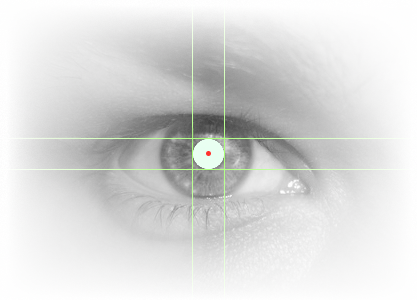
\includegraphics[width=0.60\textwidth]{images/project-iris}
\end{figure}
\vspace{0.5 in}
{\centering \huge \color{accentcolor} \sc \textbf{\teamname \\ \productname} \par}
\vspace{0.5 in}
{\centering \large \sc \textbf{\authors} \par}
\newpage


%\vspace{1 in}
%\centerline{January 13th, 2012}
%\newpage

%%% Revision History
\begin{versionhistory}
	\vhEntry{0.1}{12.14.2016}{NS\textbackslash{}TS\textbackslash{}MZ\textbackslash{}SU\textbackslash{}TM}{document creation}
\end{versionhistory}
\newpage

%%% Table of contents
\setcounter{tocdepth}{2}
\tableofcontents
\newpage

%%% List of figures and tables (optional)
\listoffigures
\listoftables
\newpage

%%% Document sections
\section{Introduction}
Your introduction should provide a brief overview of the product concept and a reference to the requirement specification and architectural design documents in 1 or 2 paragraphs. The purpose is to provide the reader with the location of relevant background material that lead to the design details presented in this document.

\newpage
\section{System Overview}
This section should describe the overall structure of your software system. Think of it as the strategy for how you will build the system. An architectural "layer" is the top-level logical view, or an abstraction, of your design. Layers should be composed of related elements of similar capabilities, and should be highly independent of other layers, but should have very clearly defined interfaces and interactions with other layers. Each layer should be identified individually and should be unique as to its function and purpose within the system. This section should also contain the high-level block diagram of the layers, as shown in the example below, as well as detailed descriptions of the functions of each layer.

\begin{figure}[h!]
	\centering
 	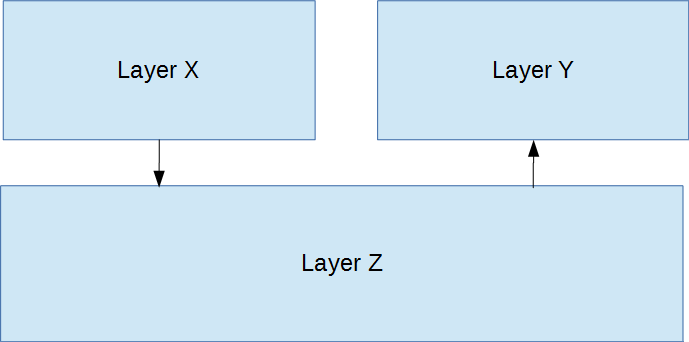
\includegraphics[width=0.60\textwidth]{images/layers}
 \caption{A simple architectural layer diagram}
\end{figure}

\subsection{Layer X Description}
Each layer should be described separately in detail. Descriptions should include the features, functions, critical interfaces and interactions of the layer. The description should clearly define the services that the layer provides. Also include any conventions that your team will use in describing the structure: naming conventions for layers, subsystems, modules, and data flows; interface specifications; how layers and subsystems are defined; etc. 

\subsection{Layer Y Description}
Each layer should be described separately in detail. Descriptions should include the features, functions, critical interfaces and interactions of the layer. The description should clearly define the services that the layer provides. Also include any conventions that your team will use in describing the structure: naming conventions for layers, subsystems, modules, and data flows; interface specifications; how layers and subsystems are defined; etc. 

\subsection{Layer Z Description}
Each layer should be described separately in detail. Descriptions should include the features, functions, critical interfaces and interactions of the layer. The description should clearly define the services that the layer provides. Also include any conventions that your team will use in describing the structure: naming conventions for layers, subsystems, modules, and data flows; interface specifications; how layers and subsystems are defined; etc. 
\newpage
\section{Subsystem Definitions \& Data Flow}
Project Iris will use a series of interfaces on each of it's layers in order to facilitate communications between them. Each layer will be implemented independently and relie on their stable interfaces to communicate information.

\begin{figure}[h!]
	\centering
 	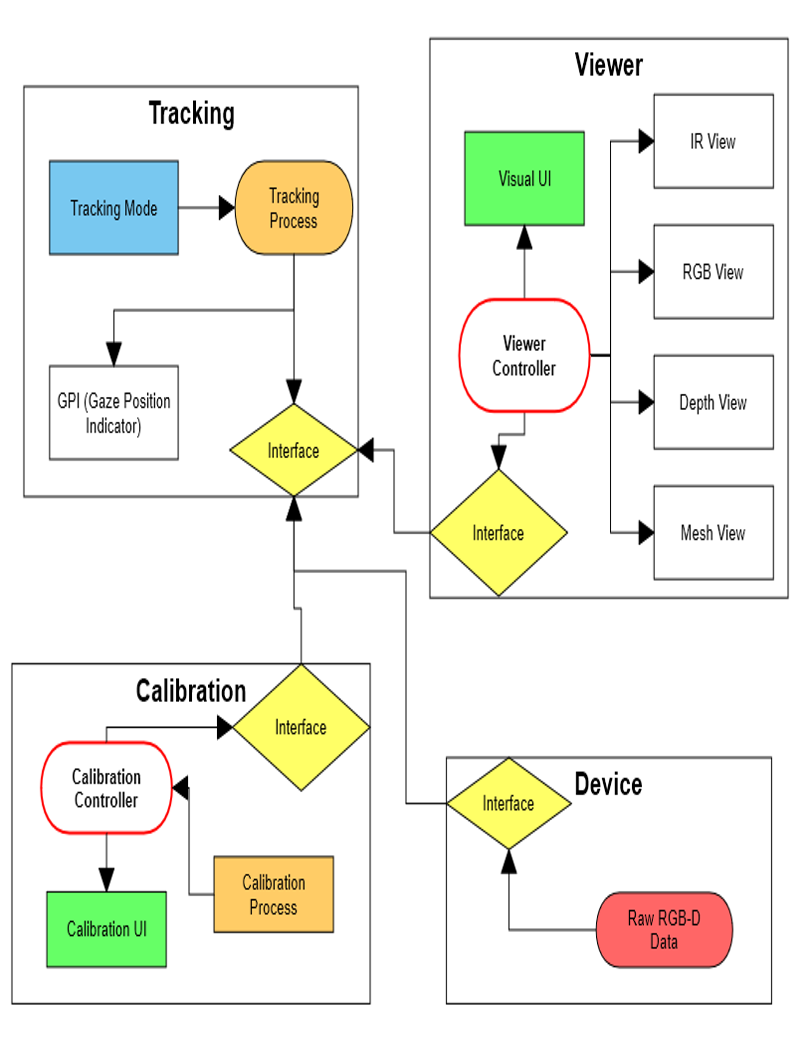
\includegraphics[width=\textwidth]{images/system-architecture}
 \caption{A simple data flow diagram}
\end{figure}

\newpage
\section{Tracking Subsystems}
The tracking layer will consist of three subsystems and an interface. These subsystems are the tracking mode, tracking process, and GPI (Gaze Position Indicator).

\begin{figure}[h!]
	\centering
	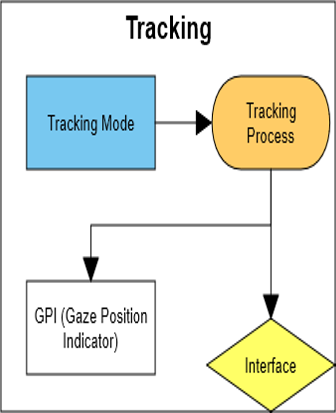
\includegraphics[width=0.60\textwidth]{images/tracking}
	\caption{Example subsystem description diagram}
\end{figure}

\subsection{Tracking Mode}
The tracking mode primarily consist of two states. Either controlling the cursor, or simply returning a set of screen coordinates that indicate the gaze position on the screen.

\subsubsection{Assumptions}
Project Iris has assumed that windows is the operating system being used, and that it's mousing API will not change significantly.

\subsubsection{Responsibilities}
It is this layers responsibility to determine if a set of coordinates are made available for API calls, or if the tracking algorithm is actively updating the systems mouse position.

\subsubsection{Subsystem Interfaces}

\begin {table}[H]
\caption {Subsystem interfaces} 
\begin{center}
    \begin{tabular}{ | p{1cm} | p{6cm} | p{3cm} | p{3cm} |}
    \hline
    ID & Description & Inputs & Outputs \\ \hline
    \#1 & Tracking Mode/Tracking Process & \pbox{3cm}{ } & \pbox{3cm}{Mode}  \\ \hline
    \end{tabular}
\end{center}
\end{table}

\subsection{Tracking Process}
The tracking process is the most important subsystem in all of Project Iris. It is where the gaze tracking algorithm will reside and also system updating will occur. The tracking process will calculate the position on screen based on gathered eye point data.  It will then use a smoothing algorithm to filter noise by using a quadratic technique to remove jitter.  Once after smoothed, if any point is calculated outside of the client window, the boundaries of the point are then recaculated to adjust to screen size.  If any point is greater than 30 degree angle of gaze then those gaze points will not be caculated and it will use the previous frame's position.

\subsubsection{Responsibilities}
It is this layers responsibility to actively track the users gaze position using data from the device layer and mode information from the mode layer.

\subsubsection{Subsystem Interfaces}

\begin {table}[H]
\caption {Subsystem interfaces} 
\begin{center}
	\begin{tabular}{ | p{1cm} | p{6cm} | p{3cm} | p{3cm} |}
		\hline
		ID & Description & Inputs & Outputs \\ \hline
		\#1 & Tracking Process/Tracking Mode & \pbox{3cm}{Mode} & \pbox{3cm}{ }  \\ \hline
		\#2 & Tracking Process/Interface & \pbox{3cm}{Raw Data\\Settings Changes} & \pbox{3cm}{Status}  \\ \hline
	\end{tabular}
\end{center}\textsl{}
\end{table}

\subsection{GPI (Gaze Position Indicator)}
The GPI subsystem will take the position provided by the tracking process and display a green graphical dot on the screen that indicates position.

\subsubsection{Subsystem Interfaces}

\begin {table}[H]
\caption {Subsystem interfaces} 
\begin{center}
	\begin{tabular}{ | p{1cm} | p{6cm} | p{3cm} | p{3cm} |}
		\hline
		ID & Description & Inputs & Outputs \\ \hline
		\#1 & Tracking Process/GPI & \pbox{3cm}{Gaze position} & \pbox{3cm}{ }  \\ \hline
	\end{tabular}
\end{center}
\end{table}


\newpage
\section{Viewer Subsystems}
The viewer layer makes up the UI of Project Iris. It will expose settings and raw data to the user to facilitate a better understanding of what is taking place behind the scenes.

\begin{figure}[h!]
	\centering
	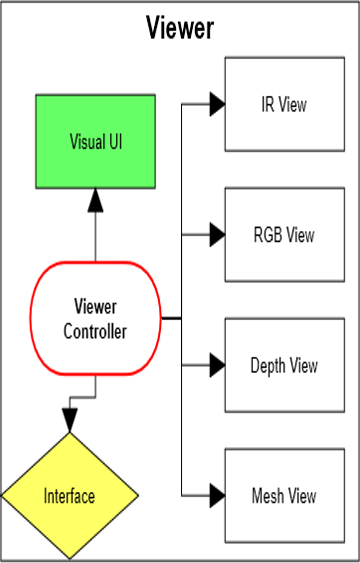
\includegraphics[width=0.60\textwidth]{images/viewer}
	\caption{Example subsystem description diagram}
\end{figure}

\subsection{Visual UI}
The visual UI is the main component of Project Iris that a user will see. It allows the user to change mode, calibrate the software, and see the raw data generated by the software. All changes will then go through the controller.

\subsubsection{Assumptions}
The UI will be built using windows 10 APIs.

\subsubsection{Subsystem Interfaces}

\begin {table}[H]
\caption {Subsystem interfaces} 
\begin{center}
    \begin{tabular}{ | p{1cm} | p{6cm} | p{3cm} | p{3cm} |}
    \hline
    ID & Description & Inputs & Outputs \\ \hline
    \#1 & UI/Controller & \pbox{3cm}{Device Data\\Software State} & \pbox{3cm}{User Selections}  \\ \hline
    \end{tabular}
\end{center}
\end{table}

\subsection{Viewer Controller}
The controller is where an algorithms or data changes the UI needs to make are accomplished. This will facilitate seperating the Windows UI elements from the rest of Project Iris and should improve the ability of the project to be ported later.

\subsubsection{Responsibilities}
This subsystem is responsible for updating the Tracking layer, calling the calibration utility, and ensuring important events are relayed to the user.

\subsubsection{Subsystem Interfaces}

\begin {table}[H]
\caption {Subsystem interfaces} 
\begin{center}
	\begin{tabular}{ | p{1cm} | p{6cm} | p{3cm} | p{3cm} |}
		\hline
		ID & Description & Inputs & Outputs \\ \hline
		\#1 & Controller/UI & \pbox{3cm}{User Selections} & \pbox{3cm}{Device Data \\Software State}  \\ \hline
		\#2 & Viewer interface & \pbox{3cm}{Device Data\\System Events\\Software State} & \pbox{3cm}{Settings Changes\textsl{}}  \\ \hline
	\end{tabular}
\end{center}
\end{table}

\newpage
\section{Calibration Subsystems}
The calibration layer is responsible for the calibration of the software to a specific user. This data is crucial to obtaining acurate gaze tracking information and displaying it for the user/system.

\begin{figure}[h!]
	\centering
	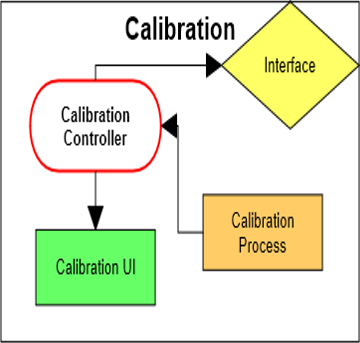
\includegraphics[width=0.60\textwidth]{images/calibration}
	\caption{Example subsystem description diagram}
\end{figure}

\subsection{Calibration UI}
The calibration UI displays information to the user so that that the calibration process can calculate accurate data. This is achieved by moving a dot around on the screen for the user to follow with their eyes.

\subsubsection{Assumptions}
The os of the system the UI is displayed on will be windows 10.

\subsubsection{Responsibilities}
This subsystem must accurately display the dot on the screen at the proper place and for the appropriate amount of time.

\subsubsection{Subsystem Interfaces}

\begin {table}[H]
\caption {Subsystem interfaces} 
\begin{center}
    \begin{tabular}{ | p{1cm} | p{6cm} | p{3cm} | p{3cm} |}
    \hline
    ID & Description & Inputs & Outputs \\ \hline
    \#1 & Controller/UI & \pbox{3cm}{Begin} & \pbox{3cm}{N/A}  \\ \hline
    \end{tabular}
\end{center}
\end{table}

\subsection{Calibration Process}
The calibration process receives camera information via its controller, and information about when the UI subsystem began in order to build accurate calibration information about the user.

\subsubsection{Assumptions}
The UI always performs its task in the alloted time-frame expected by the calibration process.

\subsubsection{Responsibilities}
Build accurate calibration data about the user.

\subsubsection{Subsystem Interfaces}

\begin {table}[H]
\caption {Subsystem interfaces} 
\begin{center}
	\begin{tabular}{ | p{1cm} | p{6cm} | p{3cm} | p{3cm} |}
		\hline
		ID & Description & Inputs & Outputs \\ \hline
		\#1 & Calibration Process/Controller & \pbox{3cm}{Camera Data \\ Begin} & \pbox{3cm}{Calibration File}  \\ \hline
	\end{tabular}
\end{center}
\end{table}

\subsection{Subsystem 3}
The calibration controller is responsible for coordinating the beginning of the calibration process, passing information to the calibration process, and ensuring the delivery of calibration data back to the rest of the system. This model allows the UI or Process to change independently of each other, all while maintaining a seamless interface for the rest of the system.

\subsubsection{Responsibilities}
Begin the calibration process in a timely manner and return accurate calibration data to the rest of the system.

\subsubsection{Subsystem Interfaces}

\begin {table}[H]
\caption {Subsystem interfaces} 
\begin{center}
	\begin{tabular}{ | p{1cm} | p{6cm} | p{3cm} | p{3cm} |}
		\hline
		ID & Description & Inputs & Outputs \\ \hline
		\#1 & Controller/interface & \pbox{3cm}{Device Data \\ Begin} & \pbox{3cm}{Calibration File}  \\ \hline
		\#2 & Controller/UI & \pbox{3cm}{N/A} & \pbox{3cm}{Begin}  \\ \hline
		\#3 & Controller/Process & \pbox{3cm}{Calibration Data} & \pbox{3cm}{Begin \\ Device Data}  \\ \hline
	\end{tabular}
\end{center}
\end{table}


\newpage
\section{Device Subsystems}
The device layer is the simplest layer in the system, and consist of the drivers for the SR300 and the interface for it.

\begin{figure}[h!]
	\centering
	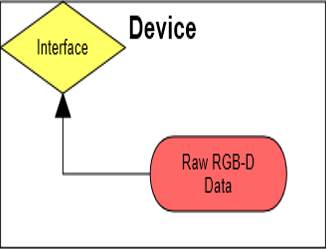
\includegraphics[width=0.60\textwidth]{images/device}
	\caption{Example subsystem description diagram}
\end{figure}

\subsection{Data}
The data subsystem only sends its data out to the interface.

\subsubsection{Subsystem Interfaces}

\begin {table}[H]
\caption {Subsystem interfaces} 
\begin{center}
    \begin{tabular}{ | p{1cm} | p{6cm} | p{3cm} | p{3cm} |}
    \hline
    ID & Description & Inputs & Outputs \\ \hline
    \#xx & Data/Interface & \pbox{3cm}{N/A} & \pbox{3cm}{Data Stream}  \\ \hline
    \end{tabular}
\end{center}
\end{table}


\newpage

%%% References
\bibliographystyle{plain}
\bibliographystyle{reference/IEEEtran_custom}
\bibliography{reference/refs}{}

\end{document}